\documentclass{beamer}
\usepackage{subfigure}
\usepackage{amssymb, amsmath, amsfonts,verbatim}
\usepackage{tikz}
\graphicspath{ {./} }
\usetikzlibrary{matrix,arrows,fit,backgrounds,mindmap,plotmarks,decorations.pathreplacing}

\usepackage{pgfplots}
\pgfplotsset{compat=1.12}
\pgfdeclarelayer{background}
\pgfsetlayers{background,main}

\tikzset{decoration={name=none},}

\newlength\figureheight
\newlength\figurewidth


\newcommand{\tikzdir}[1]{#1.tikz}
\newcommand{\inputtikz}[1]{\input{\tikzdir{#1}}}

\newcommand{\tI}{\tilde {\mathcal I}}
\newcommand{\tA}{\tilde A}
\newcommand{\ty}{\tilde y}
\newcommand{\tx}{\tilde x}
\newcommand{\tw}{\tilde w}
\newcommand{\tv}{\tilde v}
\newcommand{\tC}{\tilde C}
\newcommand{\tP}{\tilde P}
\newcommand{\Ic}{{\mathcal I^c}}
\newcommand{\J}{{\mathcal J}}
\newcommand{\K}{{\mathcal K}}


\DeclareMathOperator{\Smin}{Smin}
\DeclareMathOperator{\Smid}{Smid}
\DeclareMathOperator{\Smax}{Smax}
\DeclareMathOperator{\MSE}{MSE}
\DeclareMathOperator{\rank}{rank}
\DeclareMathOperator{\Med}{Med}
\DeclareMathOperator{\Max}{Max}
\DeclareMathOperator{\Min}{Min}
\DeclareMathOperator{\tr}{tr}
\DeclareMathOperator{\Cov}{Cov}
\DeclareMathOperator{\logdet}{log\;det}
\DeclareMathOperator{\argmin}{arg\;min}
\DeclareMathOperator{\argmax}{arg\;max}
\let\Tiny\tiny

\mode<presentation>

\title[Secure Info Fusion]{Secure Information Fusion in Cyber-Physical Systems}
\author[Yilin Mo]{Yilin Mo}
\institute[NTU]{
  School of EEE\\ Nanyang Technological University\\
}
\date[Dec 11, 2016]{Workshop on Rich Data Backed Control and Optimization for Smart Cities \\ \vspace{1cm}
  \small Joint Work with Duo Han, Xinghua Liu, \\
  Richard M. Murray, Lihua Xie and Emanuele Garone}
\usetheme{CambridgeUS}
\useinnertheme{circles}
\useoutertheme{infolines}
\definecolor{caltechcolor}{RGB}{0,52,120}
\definecolor{mycolor1}{RGB}{1.00000,0.00000,1.00000}
\usecolortheme[RGB={0,52,120}]{structure} 
\setbeamercolor*{palette primary}{fg=caltechcolor!60!black,bg=gray!30!white}
\setbeamercolor*{palette secondary}{fg=caltechcolor!70!black,bg=gray!15!white}
\setbeamercolor*{palette tertiary}{bg=caltechcolor!80!black,fg=gray!10!white}
\setbeamercolor*{palette quaternary}{fg=caltechcolor,bg=gray!5!white}
\setbeamercolor{titlelike}{parent=palette primary,fg=caltechcolor}

\begin{document}

\begin{frame}
  \titlepage
\end{frame}


\section{Introduction}

\begin{frame}{Cyber-Physical System}
  \begin{itemize}
  \item Cyber-Physical Systems (CPSs) refer to the embedding of computation, communication and control into physical spaces.
    \begin{center}
      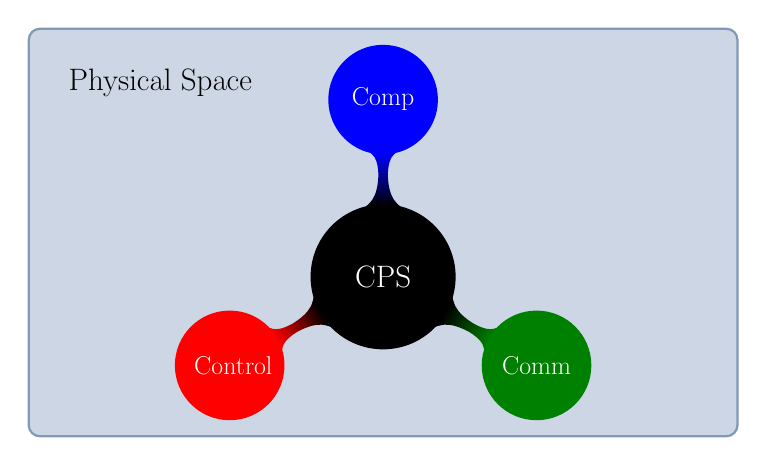
\begin{tikzpicture}[scale=0.45,transform shape,level distance=0cm,
        level 1 concept/.append style={sibling angle=120,minimum size = 3cm},
        ]
        \path [draw=caltechcolor!50,fill=caltechcolor!20,thick,rounded corners] (-10,-4.5) rectangle (10,7);
        \node at (-9,6) [anchor=north west] {\Huge Physical Space};
        \path[mindmap,concept color=black,text=white]
        node[concept] {\Huge CPS}
        [clockwise from=330]
        child[concept color=green!50!black] { node[concept](communication) {\huge Comm} }
        child[concept color=red] { node[concept](control) {\huge Control} }
        child[concept color=blue] { node[concept](computation) {\huge Comp} };
      \end{tikzpicture}
    \end{center}
  \item Applications: aerospace, chemical processes, civil infrastructure, energy, manufacturing and transportation. 
  \end{itemize}
\end{frame}

\begin{frame}{Security Threats for the CPS}
  \begin{itemize}
  \item The next generation CPS: Smart Grids, Smart Buildings, Smart Home, Internet of Things, will make extensive use of widespread sensing and networking.
  \item As the CPSs become ``smarter'', they are also more vulnerable to malicious attacks.
  \end{itemize}
  \begin{figure}[ht]
    \centering
    \includegraphics[width=0.6\textwidth]{SmartHome.jpg}
  \end{figure}
\end{frame}

\begin{frame}{Stuxnet}
  \begin{figure}[ht]
    \centering
    \includegraphics[width=0.8\textwidth]{stuxnet.jpg}
  \end{figure}
  Stuxnet is the first discovered malware that spies on and subverts industrial control systems. It was discovered in June 2010. 
\end{frame}

\begin{frame}{Industrial Control Systems}
  \begin{figure}[ht]
    \centering
    \includegraphics[width=0.6\textwidth]{cert.jpg}
  \end{figure}
 In FY 2014, ICS-CERT (Industrial Control Systems Cyber Emergency Response Team) received and responded to 245 incidents as reported by asset owners and industry partners.
\end{frame}


\begin{frame}{Industrial Control Systems}
   The scope of incidents encompassed a vast range of threats and observed methods for attempting to gain access to both business and control systems infrastructure, including but not limited to the following:
  \begin{enumerate}
  \item  Unauthorized access and exploitation of Internet facing ICS/Supervisory Control and Data Acquisition (SCADA) devices,
  \item 	 Exploitation of zero-day vulnerabilities in control system devices and software, 
  \item  	 Malware infections within air-gapped control system networks,
  \item \dots
  \end{enumerate}

\end{frame}

\begin{frame}{Attack Through Compromised Supply Chain}
  \begin{figure}[ht]
    \centering
    \includegraphics[width=0.8\textwidth]{boeing.jpg}
    \caption{Boeing 787 outsourced 70\% of its parts.}
  \end{figure}
\end{frame}

\begin{frame}{2003 Northeast Blackout}
  \begin{figure}[<+htpb+>]
    \begin{center}
      \includegraphics[width=0.60\textwidth]{blackout.jpg}
      \caption{A successful attack on CPS can have devastating effects.}
    \end{center}
  \end{figure}
\end{frame}

\begin{frame}{How to deal with CPS security threats}
  \begin{exampleblock}{}
    {\it `` If you know the enemy and know yourself, you need not fear the result of a hundred battles. If you know yourself but not the enemy, for every victory gained you will also suffer a defeat. If you know neither the enemy nor yourself, you will succumb in every battle.''}
    \vskip5mm
    \hspace*\fill{ \small--- The Art of War }
  \end{exampleblock}

  \begin{enumerate}
  \item Intrusion detection and isolation
  \item Information Fusion 
  \end{enumerate}
\end{frame}

%\begin{frame}{Overview of My Research in CPS}
%\begin{block}{Networked Control System}
%  Understanding the interaction between control and communication.
% \begin{itemize}
%  \item Kalman filtering with intermittent observation
%  \item Sensor/Actuator Scheduling: offline-schedules and event-based schedules.
%  \item Energy efficiency of consensus algorithm
% \end{itemize}
%\end{block}
%\begin{block}{CPS Security}
%\begin{itemize}
%  \item Replay attack: we proposed countermeasures to Stuxnet one year before its discovery
%  \item Deception attack
%  \item CPS security and electricity market
%  \item Information fusion
%\end{itemize}
%\end{block}

  
%\end{frame}


%\section{Secure State Estimation}
%\frame{\tableofcontents[currentsection]}
\begin{frame}{Preliminary: Static State Estimation}
  \begin{enumerate}
  \item We assume that $x \in \mathbb R^n$ is the state that we want to estimate.
  \item $m$ sensors are deployed to monitor the system. Denote $z_i \in \mathbb R$ as the measurement generated by sensor $i$.
  \item Denote $z = \begin{bmatrix}z_1&\dots&z_m\end{bmatrix}^T$ as the collection of all sensory data.
  \item We assume the following sensor model:
    \begin{align*}
      z = Hx + w,
    \end{align*}
    where $H$ is a matrix of proper dimension and $w$ represent random noise.
  \item The optimal state estimator is of the form
    \begin{align*}
      \hat x = Kz, \text{ where }K = (H^TH)^{-1}H^T.
    \end{align*}
  \end{enumerate}
\end{frame}

\begin{frame}{Preliminary: Secure State Estimation}
  Suppose the following sensory model:
  \begin{align*}
    y = \begin{bmatrix}
      1\\
      1\\
      1
    \end{bmatrix}x + w.
  \end{align*}
  The optimal estimator is given by
  \begin{align*}
    \hat x = \frac{1}{3}\left(y_1+y_2+y_3\right).
  \end{align*}
  
  This estimator is not resilient to a single malicious sensor.
\end{frame}

\begin{frame}{Problem Formulation}
  \begin{enumerate}
  \item Assume that at most $p$ sensors are compromised.
  \item The sensory model is given by
    \begin{align*}
      y = z + a = Hx + w +a,
    \end{align*}
    where $a$ is a $p$-sparse vector indicating the attacker's action.
  \item We will call an estimator $\hat x = g(y)$ to be resilient if
    \begin{align*}
      \|g(y) - g(z)\|\text{ is bounded for all $p$-sparse $a$}.
    \end{align*}
  \item The total state estimation error can be written as
    \begin{align*}
      x-g(y) = x-g(z) + g(z)-g(y).
    \end{align*}

    \emph{Resiliency means that the state estimation error caused by the adversary is bounded!}
  \end{enumerate}
\end{frame}

\begin{frame}{Why do not use information security}
  \begin{itemize}
  \item Tamper-resistant microprocessor, Software attestation, Secure Communication Protocol,\dots
  \item It is hard to guarantee security for every single sensor. (A single compromised sensor can totally ruin the linear estimator.)
  \item Physical attacks?
  \item A resilient estimator can provide an additional layer of protection.
  \end{itemize}
\end{frame}

\begin{frame}{Why not use bad data detection?}
  \begin{figure}[ht]
    \centering
    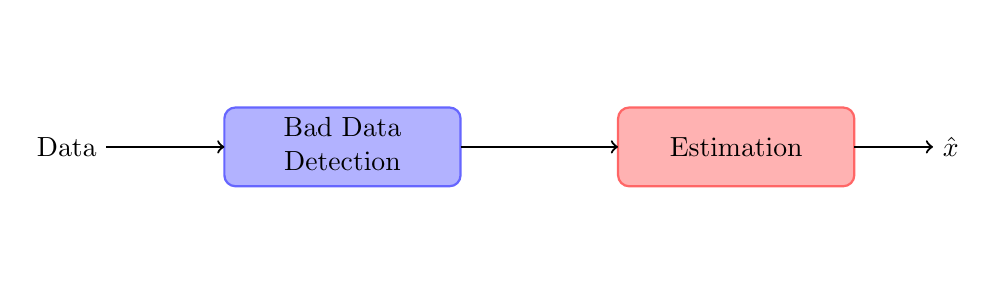
\begin{tikzpicture}
      \draw[thick,rounded corners,fill=white!30,draw=white!60] (-0.5,0) rectangle (8.5,3);

      \draw[thick,rounded corners,fill=blue!30,draw=blue!60] (0,1) rectangle (3,2);
      \node at (1.5,1.5) {\begin{tabular}{c} Bad Data\\ Detection \end{tabular}};

      \draw[thick,rounded corners,fill=red!30,draw=red!60] (5,1) rectangle (8,2);
      \node at (6.5,1.5) {Estimation};

      \draw[thick,->] (-1.5,1.5)--(0,1.5);
      \node [anchor=east] at (-1.5,1.5) {Data};

      \draw[thick,->] (3,1.5) to (5,1.5);

      % \draw[thick,->] (1.5,2) to [bend left] (6.5,2);
      % \draw[thick,->] (6.5,1) to [bend left] (1.5,1);

      \draw[thick,->] (8,1.5) to (9,1.5);

      \node [anchor=west] at (9,1.5) {$\hat x$};
    \end{tikzpicture}
    \caption{Bad Data Detection Scheme}
  \end{figure}
  \begin{enumerate}
  \item A typical bad data detector will first compute $\hat x = Ky$ and then the residue $r = y - H\hat x$.
  \item The bad data detector will then remove the sensors with large residue.
  \item Drawbacks: It is designed for \emph{random failures}, not necessarily attacks; Difficult to analyze the estimation performance.
  \end{enumerate}
\end{frame}

\begin{frame}{Why not use bad data detection?}
  \begin{figure}[ht]
    \centering
    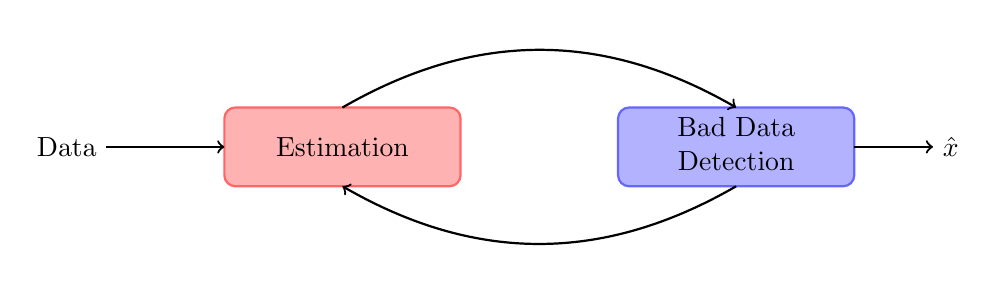
\begin{tikzpicture}
      \draw[thick,rounded corners,fill=white!30,draw=white!60] (-0.5,0) rectangle (8.5,3);

      \draw[thick,rounded corners,fill=red!30,draw=red!60] (0,1) rectangle (3,2);
      \node at (1.5,1.5) {Estimation};

      \draw[thick,rounded corners,fill=blue!30,draw=blue!60] (5,1) rectangle (8,2);
      \node at (6.5,1.5) {\begin{tabular}{c} Bad Data\\ Detection \end{tabular}};

      \draw[thick,->] (-1.5,1.5)--(0,1.5);
      \node [anchor=east] at (-1.5,1.5) {Data};

      % \draw[thick,->] (3,1.5) to (5,1.5);

      \draw[thick,->] (1.5,2) to [bend left] (6.5,2);
      \draw[thick,->] (6.5,1) to [bend left] (1.5,1);

      \draw[thick,->] (8,1.5) to (9,1.5);

      \node [anchor=west] at (9,1.5) {$\hat x$};
    \end{tikzpicture}
    \caption{Bad Data Detection Scheme}
  \end{figure}
  \begin{enumerate}
  \item A typical bad data detector will first compute $\hat x = Ky$ and then the residue $r = y - H\hat x$.
  \item The bad data detector will then remove the sensors with large residue.
  \item Drawbacks: It is designed for \emph{random failures}, not necessarily attacks; Difficult to analyze the estimation performance.
  \end{enumerate}
\end{frame}

\begin{frame}{Some Related Research}
  \begin{enumerate}
    % \item For the noiseless case, i.e., $w = 0$ we know that
    %   \begin{itemize}
    %   \item If for any $x\neq 0$, $\|Hx\|_0 \geq p+1$, then we can detect the existence of compromised sensors.
    %   \item If for any $x\neq 0$, $\|Hx\|_0 \geq 2p+1$, then we can isolate the set of compromised sensors and reconstruct $x$.
    %   \end{itemize}
  \item The following estimator is resilient:
    \begin{align*}
      & \mathop{\textit{minimize}}\limits_{\hat x,a,w}&
      & \|w\|^2 \\
      &\text{subject to}&
      &y = H \hat x + w + a,\,\|a\|_0\leq p.
    \end{align*}
    The drawback: The optimization problem is not convex and solving it is computationally difficult.
  \item We can use convex optimization based estimator, e.g., 
    \begin{align*}
      & \mathop{\textit{minimize}}\limits_{\hat x,a,w}&
      & \|w\|^2 + \|a\|_1 \\
      &\text{subject to}&
      &y = H \hat x + w + a.
    \end{align*}
    However, there is no guarantee on the resiliency.
  \end{enumerate}
\end{frame}

\begin{frame}{A General Convex Optimization Based Estimator}
  We consider the following estimator
  \begin{align*}
    \hat x = g(y) \triangleq \argmin_{\hat x} \sum_{i=1}^m f_i(y_i-H_i \hat x),
  \end{align*}
  where the following properties of function $f_i:\mathbb R\mapsto \mathbb R$ are assumed:
  \begin{enumerate}
  \item $f_i$ is convex.
  \item $f_i$ is symmetric, i.e., $f_i(u) = f_i(-u)$.
  \item $f_i$ is non-negative and $f_i(0) = 0$.
  \end{enumerate} 

  If we define the residue $r_i\triangleq y_i - H_i\hat x$, then we are trying to minimize the sum of some cost function related to the residue.

  The estimator can be computed efficiently via convex optimization. (It is also easy be computed in a parallel fashion.)
\end{frame}


\begin{frame}{A General Convex Optimization Based Estimator}
  Our proposed estimator is very general since we can choose the right $f_i$ to get the following estimator:
  \begin{enumerate}
  \item Linear Estimator:
    \begin{align*}
      g(y) = \argmin_{\hat x} \|y-H\hat x\|_2^2= \argmin_{\hat x}  \sum_{i=1}^m (y_i-H_i\hat x)^2.
    \end{align*}
  \item $L_1$ Estimator:
    \begin{align*}
      g(y) = \argmin_{\hat x} \|y-H\hat x\|_1=\argmin_{\hat x} \sum_{i=1}^m |y_i-H_i\hat x|.
    \end{align*}
  \end{enumerate}
\end{frame}


\begin{frame}{A General Convex Optimization Based Estimator}
  \begin{enumerate}  \setcounter{enumi}{2}

  \item LASSO:
    \begin{align*}
      g(y) = \argmin_{\hat x} \|w\|^2+\lambda \|a\|_1, \text{ s.t. }y=H\hat x+w+a.
    \end{align*}
    We can define $r_i = y_i-H_i\hat x = w_i+a_i$. Then the problem can be rewritten as
    \begin{align*}
      g(y) = \argmin_{\hat x}\sum_{i=1}^m \min_{w_i}\left(\|w_i\|^2+\lambda \|r_i-w_i\|_1\right), \text{ s.t. }r_i=y_i-H\hat x.
    \end{align*}
    As a result, we can rewrite $g$ as
    \begin{align*}
      g(y) = \argmin_{\hat x} \sum_{i=1}^m f(y_i-H_i\hat x)
    \end{align*}
    where $f(r) = \min_{w} w^2 + \lambda |r-w|.$
  \end{enumerate}
\end{frame}

\begin{frame}{Example}
  Suppose the following sensory model:
  \begin{align*}
    y = \begin{bmatrix}
      1\\
      1\\
      1
    \end{bmatrix}x + w+a,\,\|a\|_0\leq 1.
  \end{align*}
  Then the following estimator is resilient (in fact, it is the median of $y_i$):
  \begin{align*}
    g(y) = \argmin_{\hat x}  |y_1-\hat x|+|y_2-\hat x|+|y_3-\hat x|.
  \end{align*}
\end{frame}

\begin{frame}{Example}
  \begin{figure}[ht]
    \centering
    \begin{tikzpicture}[yscale=0.4]
      \draw[thick,->] (0,0)--(9,0);
      \node [anchor=west] at (9,0) {$\hat x$};
      \draw[thin,gray] (2,0)--(2,0.1);
      \draw[thin,gray] (5,0)--(5,0.1);
      \draw[thin,gray] (7,0)--(7,0.1);
      \draw[thick](1,11)--(2,8)--(5,5)--(7,7)--(8,10);
      \node [anchor=north] at (2,0) {\color{red}{$y_1$}};
      \node [anchor=north] at (5,0) {\color{blue}{$y_2$}};
      \node [anchor=north] at (7,0) {\color{brown}{$y_3$}};
    \end{tikzpicture}
  \end{figure}
  \color{white}{If we interpret the function $|y_i-\hat x|$ as a potential function generate by sensor $i$, then we can see that sensor $i$ is dragging $\hat x$ towards $y_i$ with $1$ unit of force. The equilibrium point will be at the middle $y_i$.}
\end{frame}

\begin{frame}{Interpretation}
  \begin{figure}[ht]
    \centering
    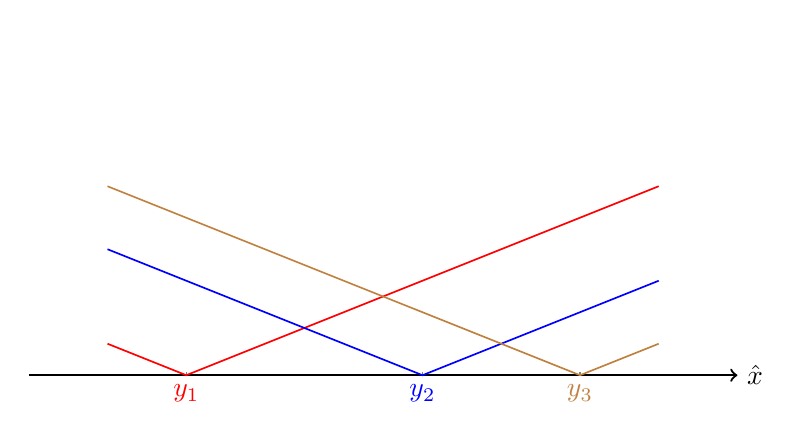
\begin{tikzpicture}[yscale=0.4]
      \draw[thick,->] (0,0)--(9,0);
      \node [anchor=west] at (9,0) {$\hat x$};
      \draw[thin,gray] (2,0)--(2,0.1);
      \draw[thin,gray] (5,0)--(5,0.1);
      \draw[thin,gray] (7,0)--(7,0.1);
      \draw[thick,white](1,11)--(2,8)--(5,5)--(7,7)--(8,10);
      \node [anchor=north] at (2,0) {\color{red}{$y_1$}};
      \draw[semithick,red](1,1)--(2,0)--(8,6);
      \node [anchor=north] at (5,0) {\color{blue}{$y_2$}};
      \draw[semithick,blue](1,4)--(5,0)--(8,3);
      \node [anchor=north] at (7,0) {\color{brown}{$y_3$}};
      \draw[semithick,brown](1,6)--(7,0)--(8,1);
    \end{tikzpicture}
  \end{figure}
  If we interpret the function $|y_i-\hat x|$ as a potential function generate by sensor $i$, then we can see that sensor $i$ is dragging $\hat x$ towards $y_i$ with $1$ unit of force. The equilibrium point will be at the middle $y_i$.
\end{frame}

\begin{frame}{Another Example}
  Suppose the following sensory model:
  \begin{align*}
    y = \begin{bmatrix}
      1\\
      1\\
      3
    \end{bmatrix}x + w+a ,\,\|a\|_0\leq 1.
  \end{align*}
  Then the following estimator is not resilient:
  \begin{align*}
    g(y) = \argmin_{\hat x}  |y_1-\hat x|+|y_2-\hat x|+|y_3-3\hat x|.
  \end{align*}
  In fact, we can rewrite it as
  \begin{align*}
    g(y) = \argmin_{\hat x}  |y_1-\hat x|+|y_2-\hat x|+3\left|\frac{y_3}{3}-\hat x\right| = \frac{y_3}{3}
  \end{align*}
  Sensor $3$ generates $3$ unit of force comparing to $1$ unit of force from sensor $1$ and $2$.
\end{frame}


\begin{frame}{Sufficient Condition For Resiliency}
  \begin{theorem}
    If the following conditions hold, then the estimation is resilient:
    \begin{enumerate}
    \item For all $i$, the following limit is well-defined:
      \begin{align*}
        \lim_{t\rightarrow\infty}\frac{f_i(t)}{t} = \alpha_i < \infty.
      \end{align*}
    \item For any $u\neq 0$ and any index set $\mathcal I$ of cardinality $p$, the following inequality hold:
      \begin{align*}
        \sum_{i\in \mathcal I} |\alpha_i H_i u| < \sum_{i\in \mathcal I^c} |\alpha_i H_i u|.
      \end{align*}
    \end{enumerate}
  \end{theorem}
  Roughly speaking $|\alpha_i H_i u|$ is the force from sensor $i$ on the direction $u$. The condition can be interpreted as the force from any $p$ sensors should be smaller than the remaining $m-p$ sensors on all direction.
\end{frame}

\begin{frame}{Necessary Condition For Resiliency}
  \begin{theorem}
    If the one of the following conditions is violated, then the estimation is not resilient:
    \begin{enumerate}
    \item There exists an $i$, such that
      \begin{align*}
        \lim_{t\rightarrow\infty}\frac{f_i(t)}{t} = \infty.
      \end{align*}
    \item There exists a $u\neq 0$ and an index set $\mathcal I$ of cardinality $p$, such that
      \begin{align*}
        \sum_{i\in \mathcal I} |\alpha_i H_i u| > \sum_{i=\mathcal I^c} |\alpha_i H_i u|.
      \end{align*}
    \end{enumerate}
  \end{theorem}
  Notice that we only have a trivial gap for the case:
  \[ \sum_{i\in \mathcal I} |\alpha_i H_i u| = \sum_{i=\mathcal I^c} |\alpha_i H_i u|.\]
\end{frame}

\begin{frame}{Simulation IEEE 14-bus System}
  \begin{figure}[ht]
    \centering
    \includegraphics[width=0.60\textwidth]{ieee14.jpg}
  \end{figure}
  We assume $p=1$ and the flow sensor on the red line is being attacked.
\end{frame}


\begin{frame}{Simulation IEEE 14-bus System}
  \begin{figure}[ht]
    \begin{center}
    
      \setlength{\figureheight}{6cm}
      \setlength{\figurewidth}{10cm}
    \definecolor{mycolor1}{rgb}{1.00000,0.00000,1.00000}%
%
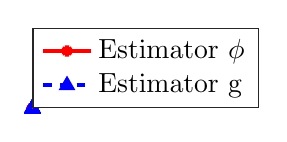
\begin{tikzpicture}

\begin{axis}[%
width=\figurewidth,
height=\figureheight,
at={(1.527in,1.083in)},
scale only axis,
xmin=0.95,
xmax=2.4,
xlabel={Normalized MSE of the estimators without attack},
xmajorgrids,
ymin=0.95,
ymax=2.5,
ylabel={Normalized MSE when under attack},
ymajorgrids,
axis background/.style={fill=white},
legend style={at={(0.597,0.528)},anchor=south west,legend cell align=left,align=left,draw=white!15!black}
]
\addplot [color=red,solid,line width=1.5pt,mark=asterisk,mark options={solid}]
  table[row sep=crcr]{%
1.43445926050949	1.60278898169176\\
1.39031186915402	1.55697434518454\\
1.3071172341038	1.45686583321128\\
1.22179873443561	1.39007675912456\\
1.19778876193304	1.39208411785897\\
1.18338657214841	1.41115912951674\\
1.19827557684201	1.43770731227953\\
1.19829876193728	1.45864622150778\\
1.19391115736641	1.47941184470539\\
1.19540182190504	1.49298640841215\\
1.21565436671202	1.5165881854638\\
1.22952576940108	1.54397316883212\\
1.2344017031641	1.57119831765969\\
1.29356861993538	1.63848995702805\\
1.49806241756897	2.01620927014096\\
};
\addlegendentry{$\text{Estimator }\phi$};

\addplot [color=blue,dashed,line width=1.5pt,mark=triangle,mark options={solid}]
  table[row sep=crcr]{%
2.16434829886514	2.41673714136766\\
1.49824142620916	1.6273922047888\\
1.46836558726546	1.61304395019434\\
1.42878218405531	1.58080265845186\\
1.33509034059386	1.48317348510781\\
1.24979953097586	1.4011442907391\\
1.20190884155895	1.36475282176979\\
1.14816845697376	1.32743887772808\\
1.104692902235	1.30458587111275\\
1.0727554366346	1.2930587844785\\
1.04837293442887	1.29286647088633\\
1.03276380632143	1.30464750437787\\
1.02491383863213	1.32636243694814\\
1.0209295289153	1.35606289076979\\
1.01470702949196	1.40680155569416\\
1.00686189169388	1.48274325705327\\
1.00166658882151	1.69020329692052\\
1.00012894457222	2.29806950301701\\
};
\addlegendentry{Estimator g};

\addplot [color=mycolor1,dashed,forget plot]
  table[row sep=crcr]{%
1	1\\
2.2	1\\
};
\addplot [color=mycolor1,dashed,forget plot]
  table[row sep=crcr]{%
1	1\\
1	2.5\\
};
\node[right, align=left, text=blue]
at (axis cs:2.164,2.417) {$\text{   }\leftarrow\text{ }\lambda\rightarrow 0$};
\node[right, align=left, text=blue]
at (axis cs:1.335,1.483) {$\text{   }\leftarrow\text{ }\lambda\text{=0.5}$};
\node[right, align=left, text=blue]
at (axis cs:1.202,1.365) {$\text{   }\leftarrow\text{ }\lambda\text{=1}$};
\node[right, align=left, text=blue]
at (axis cs:1.073,1.293) {$\text{   }\leftarrow\text{ }\lambda\text{=1.9}$};
\node[right, align=left, text=blue]
at (axis cs:1.02,1.356) {$\leftarrow\lambda\text{=3}$};
\node[right, align=left, text=blue]
at (axis cs:1,2.298) {$\text{   }\leftarrow\text{ }\lambda\text{=7}$};
\node[right, align=left, text=red]
at (axis cs:1.434,1.603) {$\text{   }\leftarrow\text{ }\epsilon\text{=0.05}$};
\node[right, align=left, text=red]
at (axis cs:1.03,1.459) {$\epsilon\text{=0.53}\rightarrow\text{   }$};
\node[right, align=left, text=red]
at (axis cs:1.498,2.016) {$\text{   }\leftarrow\text{ }\epsilon\text{=1}$};
\node[right, align=left, text=mycolor1]
at (axis cs:1,2.4) {$\text{   }\leftarrow\text{ LSE}$};
\node[right, align=left, text=mycolor1]
at (axis cs:1.9,1.14) {Oracle LSE};
\node[right, align=left, text=mycolor1]
at (axis cs:1.9,1.07) {$\text{     ~~~~~}\downarrow$};
\end{axis}
\end{tikzpicture}%

    \end{center}
  \end{figure}
\end{frame}

\begin{frame}{Dynamic State Estimation}
\begin{enumerate}
\item Consider the following dynamic system
\begin{align}
x(k+1) = A x(k) + w(k),\, y(k) = C x(k) + v(k) + a(k).
\end{align}
\item A linear fixed-gain estimator:
\begin{align}
\hat x(k+1) = A \hat x(k) + K(y(k+1)-CA\hat x(k)),
\end{align}
where $K$ is the estimation gain, and $A-KCA$ is stable.
\begin{center}
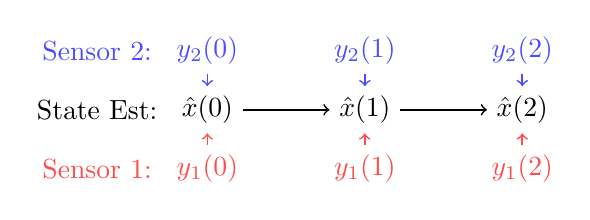
\begin{tikzpicture}[x=2cm, y=0.75cm]
\node at (-0.7,0) {State Est:};
\node [blue!70] at (-0.7,1) {Sensor 2:};
\node [red!70] at (-0.7,-1) {Sensor 1:};

\node            (x0)  at (0,0) {$\hat x(0)$};
\node [blue!70] (y20)  at (0,1)    {$y_2(0)$};
\node [red!70]  (y10)  at (0,-1)   {$y_1(0)$};
\draw [->,semithick,blue!70] (y20) to (x0);
\draw [->,semithick,red!70]  (y10) to (x0);

\node            (x1)  at (1,0) {$\hat x(1)$};
\node [blue!70] (y21)  at (1,1)    {$y_2(1)$};
\node [red!70]  (y11)  at (1,-1)   {$y_1(1)$};
\draw [->,semithick,blue!70] (y21) to (x1);
\draw [->,semithick,red!70]  (y11) to (x1);

\node            (x2)  at (2,0) {$\hat x(2)$};
\node [blue!70] (y22)  at (2,1)    {$y_2(2)$};
\node [red!70]  (y12)  at (2,-1)   {$y_1(2)$};
\draw [->,semithick,blue!70] (y22) to (x2);
\draw [->,semithick,red!70]  (y12) to (x2);

\draw [->,semithick] (x0) to (x1);
\draw [->,semithick] (x1) to (x2);
\end{tikzpicture}
\end{center}
\item The error introduced by the attack may accumulate over time.
\end{enumerate}
\end{frame}

\begin{frame}{Dynamic State Estimate: A Moving Horizon Approach}
In order to convert the dynamic estimation problem into a static one, we can use a moving horizon approach:
\begin{center}
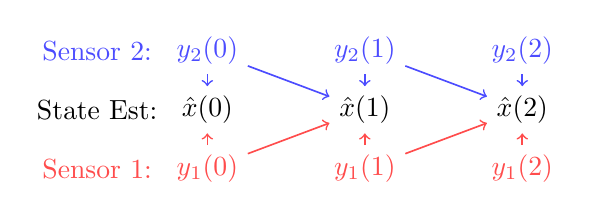
\begin{tikzpicture}[x=2cm, y=0.75cm]
\node at (-0.7,0) {State Est:};
\node [blue!70] at (-0.7,1) {Sensor 2:};
\node [red!70] at (-0.7,-1) {Sensor 1:};

\node            (x0)  at (0,0) {$\hat x(0)$};
\node [blue!70] (y20)  at (0,1)    {$y_2(0)$};
\node [red!70]  (y10)  at (0,-1)   {$y_1(0)$};
\draw [->,semithick,blue!70] (y20) to (x0);
\draw [->,semithick,red!70]  (y10) to (x0);

\node            (x1)  at (1,0) {$\hat x(1)$};
\node [blue!70] (y21)  at (1,1)    {$y_2(1)$};
\node [red!70]  (y11)  at (1,-1)   {$y_1(1)$};
\draw [->,semithick,blue!70] (y21) to (x1);
\draw [->,semithick,red!70]  (y11) to (x1);
\draw [->,semithick,blue!70] (y20) to (x1);
\draw [->,semithick,red!70]  (y10) to (x1);

\node            (x2)  at (2,0) {$\hat x(2)$};
\node [blue!70] (y22)  at (2,1)    {$y_2(2)$};
\node [red!70]  (y12)  at (2,-1)   {$y_1(2)$};
\draw [->,semithick,blue!70] (y22) to (x2);
\draw [->,semithick,red!70]  (y12) to (x2);
\draw [->,semithick,blue!70] (y21) to (x2);
\draw [->,semithick,red!70]  (y11) to (x2);
\end{tikzpicture}
\end{center}

However, the historical data are discarded and the estimation performance may be poor when the system is operating normally.
\end{frame}

\begin{frame}{Dynamic State Estimate: A Local Estimator Approach}
We propose to store historical data in the local estimations:
\begin{center}
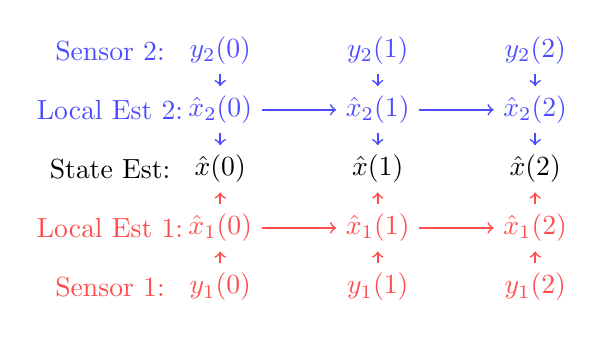
\begin{tikzpicture}[x=2cm, y=0.75cm]
\node at (-0.7,0) {State Est:};
\node [blue!70] at (-0.7,2) {Sensor 2:};
\node [blue!70] at (-0.7,1) {Local Est 2:};
\node [red!70] at (-0.7,-2) {Sensor 1:};
\node [red!70] at (-0.7,-1) {Local Est 1:};

\node            (x0)  at (0,0)    {$\hat x(0)$};
\node [blue!70] (y20)  at (0,2)       {$y_2(0)$};
\node [blue!70] (x20)  at (0,1)  {$\hat x_2(0)$};
\node [red!70]  (y10)  at (0,-2)      {$y_1(0)$};
\node [red!70]  (x10)  at (0,-1) {$\hat x_1(0)$};
\draw [->,semithick,blue!70] (y20) to (x20);
\draw [->,semithick,red!70]  (y10) to (x10);
\draw [->,semithick,blue!70] (x20) to  (x0);
\draw [->,semithick,red!70]  (x10) to  (x0);

\node            (x1)  at (1,0)    {$\hat x(1)$};
\node [blue!70] (y21)  at (1,2)       {$y_2(1)$};
\node [blue!70] (x21)  at (1,1)  {$\hat x_2(1)$};
\node [red!70]  (y11)  at (1,-2)      {$y_1(1)$};
\node [red!70]  (x11)  at (1,-1) {$\hat x_1(1)$};
\draw [->,semithick,blue!70] (y21) to (x21);
\draw [->,semithick,red!70]  (y11) to (x11);
\draw [->,semithick,blue!70] (x21) to  (x1);
\draw [->,semithick,red!70]  (x11) to  (x1);

\node            (x2)  at (2,0)    {$\hat x(2)$};
\node [blue!70] (y22)  at (2,2)       {$y_2(2)$};
\node [blue!70] (x22)  at (2,1)  {$\hat x_2(2)$};
\node [red!70]  (y12)  at (2,-2)      {$y_1(2)$};
\node [red!70]  (x12)  at (2,-1) {$\hat x_1(2)$};
\draw [->,semithick,blue!70] (y22) to (x22);
\draw [->,semithick,red!70]  (y12) to (x12);
\draw [->,semithick,blue!70] (x22) to  (x2);
\draw [->,semithick,red!70]  (x12) to  (x2);

\draw [->,semithick,blue!70] (x20) to (x21);
\draw [->,semithick,blue!70] (x21) to (x22);
\draw [->,semithick,red!70] (x10) to (x11);
\draw [->,semithick,red!70] (x11) to (x12);
\end{tikzpicture}
\end{center}
\begin{enumerate}
\item Construct local estimators (which uses only the local measurements):
\begin{align*}
\hat x_i(k) = A \hat x_i(k) + L_i (y_i(k)-CA\hat x_i(k)).
\end{align*}  
\item Reconstruct the global estimator as
\begin{align*}
\hat x(k) = g(\hat x_1(k),\ldots,\hat x_m(k)).
\end{align*}  
\end{enumerate}
\end{frame}

\begin{frame}{Local Estimator Design}
\begin{enumerate}
\item  Choose $L_i$ such that $A-L_iCA$ shares the same eigenvalues as $A-KCA$.
\begin{align*}
\hat x_i(k) = A \hat x_i(k) + L_i (y_i(k)-CA\hat x_i(k)).
\end{align*}  
\item The global estimate can be recovered as
\begin{align*}
\hat x(k) = F_1\hat x_1(k)+\dots+F_m\hat x_m(k).
\end{align*}
\item More importantly, it can be written as the solution of a quadratic programming problem:
\begin{align*}
  &\mathop{\textrm{minimize}}\limits_{\hat x(k),\hat e(k)}&
  & \frac{1}{2}\hat e(k)^T \tilde W^{-1} \hat e(k)\\
  &\textrm{subject to} &
  &\hat x_i(k)  =  \hat x(k) + \hat e_i(k),&
\end{align*}
\end{enumerate}
\end{frame}

\begin{frame}{Securing the Global Estimate}
We can secure the global estimator using LASSO:
\begin{align*}
  &\mathop{\textrm{minimize}}\limits_{\hat x(k),\hat e(k)}&
  & \frac{1}{2}\hat e(k)^T \tilde W^{-1} \hat e(k) + \gamma \sum_{i=1}^m \|\hat \nu_i(k)\|_1\\
  &\textrm{subject to} &
  &\hat x_i(k)  =  \hat x(k) + \hat e_i(k)+\hat \nu_i(k),&
\end{align*}
One can prove the following:
\begin{enumerate}
\item If there is no attack, then the LASSO will recover the original estimate if the local estimation error belongs to a polytope (scaled with $\gamma$).
\item If there is an attack and less than one half of the sensors are malicious, then the estimator is still stable.
\end{enumerate}
\end{frame}
% \section{Hypothesis Testing}
% 
% \frame{\tableofcontents[currentsection]}
% \begin{frame}{A Classical Hypothesis Testing Problem}
%   \begin{itemize}
%   \item We want to decide whether the state $\theta$ is $-1$ or $1$.
%     \begin{align*}
%       \theta=\begin{cases}
%         -1 &\text{w.p.~}0.5\\
%         +1 &\text{w.p.~}0.5\\
%       \end{cases}
%     \end{align*}
%   \item $m$ sensors are measuring the state: $z_i(k)\sim\mathcal N(\theta,1)$.
%   \item Let us define 
%     \begin{displaymath}
%       z(k) = \begin{bmatrix}z_1(k)&\dots&z_m(k)\end{bmatrix},\,Z(k) = \begin{bmatrix}z(1)&\dots&z(k)\end{bmatrix}.
%     \end{displaymath}
%   \item A detector at time $k$  is a function $f_k:\mathbb R^{mk}\rightarrow \{-1,1\}$.
%   \item A detection strategy is an infinite sequence of detectors $f = (f_1,\,f_2,\,\dots)$.
%   \end{itemize}
% \end{frame}
% 
% \begin{frame}{A Classical Hypothesis Testing Problem}
%   \begin{center}
%     \setlength{\figureheight}{2cm}
%     \setlength{\figurewidth}{10cm}
%     \inputtikz{gaussian}
%   \end{center}
%   
%   Without the attacker, it is well-known that the optimal detector with minimum detection error is a Naive Bayes Detector:
%   \begin{align*}
%     \hat \theta(k)=f_k(Z(k))=\begin{cases}
%       -1 &\text{if }\sum_{i=1}^m\sum_{t=1}^k z_i(t)/mk < 0\\
%       +1 &\text{if }\sum_{i=1}^m\sum_{t=1}^k z_i(t)/mk \geq 0\\
%     \end{cases}.
%   \end{align*}
%   
%   However, the Naive Bayes Detector is not secure. Suppose the attacker compromise one sensor. Thus, it can manipulate the summation arbitrarily. Hence, it has full control over $\hat \theta$. 
% \end{frame}
% 
% 
% \begin{frame}{Attack Model}
%   The attacker compromised $p$ sensors, the set of which is denoted as $\mathcal I$. The detector knows $p$, but does not know $\mathcal I$.
%   \begin{displaymath}
%     y(k) = z(k) + a(k),  
%   \end{displaymath}
%   where $a_i(k) = 0$ if $i\notin \mathcal I$.
%   
%   We consider different information set $\mathcal G(k)$ of the attacker at time $k$:
%   \begin{itemize}
%   \item Weak Attack Model: The attacker knows only the measurements of the compromised sensors, i.e., $\mathcal G(k) = Z_{\mathcal I}(k)$.
%   \item Strong Attack Model: The attacker knows the measurements of all sensors, i.e., $\mathcal G(k) = Z(k)$. 
%   \end{itemize}
%   The disturbance $a(k)$ depends on the information set $\mathcal Z(k)$ and $\mathcal I$: 
%   \begin{displaymath}
%     a(k) = g_k(\mathcal G(k),\mathcal I). 
%   \end{displaymath}
%   The attack strategy $g = (g_1,\,g_2,\,\dots)$.
% \end{frame}
% 
% \begin{frame}{Performance: Probability of Error}
%   \begin{itemize}
%   \item The probability of error at time $k$ is denoted as
%     \begin{displaymath}
%       P_e(k) = \max_{\mathcal I}\; P(f_k(Y(k)) \neq \theta). 
%     \end{displaymath}
%   \item Clearly, $P_e(k)$ is a function of the detection strategy $f$ and the attack strategy $g$.
%   \item  In general, for a fixed $k$, optimizing $P_e(k)$ directly (either from the system's perspective or the attacker's perspective) is difficult.
%   \item As a result, we will focus on the asymptotic performance when $k\rightarrow\infty$.
%   \end{itemize}
% \end{frame}
% 
% \begin{frame}{Chernoff Information}
%   \begin{itemize}
%   \item Suppose $m = 1$ and $p = 0$, the Naive Bayes Detector takes the following form:
%     \begin{align*}
%       \hat \theta(k)=f_k(Z(k))=\begin{cases}
%         -1 &\text{if }\sum_{t=1}^k z_1(t)/k < 0\\
%         +1 &\text{if }\sum_{t=1}^k z_1(t)/k \geq 0\\
%       \end{cases}.
%     \end{align*}
%   \item By LLN, the probability of error goes to $0$.
%   \item Moreover, it goes to $0$ exponentially fast, i.e.,
%     \begin{displaymath}
%       \lim_{k\rightarrow\infty}-\frac{\log P_e(k)}{k} = \max_{0<\alpha<1} -\log \int_{-\infty}^\infty \left(\frac{p^-(x)}{p^+(x)}\right)^\alpha p^+(x) dx = \frac{1}{2}.
%     \end{displaymath}
%   \item For general $m$ with $p = 0$, the probability of error for the Naive Bayes Detector satisfies:
%     \begin{displaymath}
%       P_e(k)\sim e^{-\frac{1}{2}mk}.
%     \end{displaymath}
%   \end{itemize}
% \end{frame}
% 
% \begin{frame}{Asymptotic Performance}
%   \begin{itemize}
%   \item In adversarial environment, let us define the rate function $I$ as
%     \begin{displaymath}
%       I = \liminf_{k\rightarrow\infty} -\frac{\log P_e(k)}{k}.
%     \end{displaymath}
%     Roughly speaking, 
%     \begin{displaymath}
%       P_e(k)\sim e^{-Ik}. 
%     \end{displaymath}
%     Larger rate implies better detection performance.
%   \item  $I$ is a function of both detection strategy $f$ and attack strategy $g$.
%   \item The detector wants to maximize $I$ while the attacker wants to minimize $I$.
%   \item Our goal is to find a Nash-equilibrium $(f^*,g^*)$, such that
%     \begin{displaymath}
%       I(f^*,g)\geq I(f^*,g^*) \geq I(f,g^*).	
%     \end{displaymath}
%   \end{itemize}
% \end{frame}
% 
% \begin{frame}{Nash-equilibrium when $m \leq 2p$}
%   \it Theorem: For both weak and strong attack model, the following strategy pair $(f^*,g^*)$ is a Nash-equilibrium with $I(f^*,g^*) = 0$:
%   \begin{block}{Attack Strategy $g^*$}
%     \begin{enumerate}
%     \item Flip $m-p$ compromised sensors' measurements.
%     \item Set the rest $2p-m$ compromised sensors' measurements to $0$. 
%     \end{enumerate}
%     For example, if $m=3$ and $p=2$, then the adversary should flip $1$ sensor and set the other sensor's readings to $0$.
%   \end{block}
%   \begin{block}{Detection Strategy $f^*$}
%     $f_k = 1$ for all $k$.
%   \end{block}
% \end{frame}
% \begin{frame}{Nash-Equilibrium when $m \geq 2p+1$}
%   We need to define the following ``summation'' functions:
%   \begin{definition}
%     Define the symmetric functions $\Smin_{2p},\,\Smid_{2p},\,\Smax_{2p}:\mathbb R^{m}\rightarrow \mathbb R$ as  
%     \begin{align*}
%       \Smin_{2p}(x_1,\ldots,x_m) &\triangleq \sum_{i=1}^{m-2p}x_i,\\
%       \Smid_{2p}(x_1,\ldots,x_m) &\triangleq \sum_{i=p+1}^{m-p}x_i,\\
%       \Smax_{2p}(x_1,\ldots,x_m) &\triangleq \sum_{i=2p+1}^{m}x_i,
%     \end{align*}
%     when $x_1\leq \dots\leq x_m$.
%   \end{definition}
% \end{frame}
% 
% \begin{frame}{Nash-Equilibrium when $m \geq 2p+1$}
%   \begin{itemize}
%   \item If $\|x' - x\|_0\leq p$, then
%     \begin{displaymath}
%       \Smin_{2p}(x) \leq \Smid_{2p}(x')\leq \Smax_{2p}(x).
%     \end{displaymath} 
%   \item Assuming $m=5$, $p = 1$:
%     \begin{center}
%       \begin{tikzpicture}[semithick,>=latex]
%         \draw [->] (0,0)--(10,0);
%         \draw plot[mark=x] coordinates{(1,0)} node [above] {$x_1$};
%         \draw plot[mark=x] coordinates{(2,0)} node [above] {$x_2$};
%         \draw plot[mark=x] coordinates{(4,0)} node [above] {$x_3$};
%         \draw plot[mark=x] coordinates{(5,0)} node [above] {$x_4$};
%         \draw plot[mark=x] coordinates{(7,0)} node [above] {$x_5$};
%         
%         \draw [->] (0,-2)--(10,-2);
%         \draw plot[mark=x] coordinates{(9,-2)} node [above] {$x_1'$};
%         \draw plot[mark=x] coordinates{(2,-2)} node [above] {$x_2'$};
%         \draw plot[mark=x] coordinates{(4,-2)} node [above] {$x_3'$};
%         \draw plot[mark=x] coordinates{(5,-2)} node [above] {$x_4'$};
%         \draw plot[mark=x] coordinates{(7,-2)} node [above] {$x_5'$};
%         
%         \draw [->,dashed] (1,0)--(1,-1)--(9,-1)--(9,-2);
%         \begin{pgfonlayer}{background}
%           \fill [fill=red!30] (3,-2.5) rectangle (8,-1.25);
%           \node at (5.5,-2.3) {$\Smid_2(x')$};
%           
%           \fill [fill=blue!30] (3,-0.5) rectangle (8,0.75);
%           \node at (5.5,-0.3) {$\Smax_2(x)$};
%         \end{pgfonlayer}
%       \end{tikzpicture}
%     \end{center}
%   \item $\Smid_{2p}$ is a more ``secure'' version of sum. 
%   \end{itemize}
% \end{frame}
% 
% 
% \begin{frame}{Nash-Equilibrium when $m \geq 2p+1$}
%   \it Theorem: For both weak and strong attack model, the following strategy pair $(f^*,g^*)$ is a Nash-equilibrium with $I(f^*,g^*) = (m-2p)/2$:
%   \begin{block}{Attack Strategy $g^*$}
%     Flip $p$ compromised sensors' measurements.
%   \end{block}
%   \begin{block}{Detection Strategy $f^*$}
%     \begin{enumerate}
%     \item For each sensor $i$, compute a local sum $ \Lambda_i(k) = \sum_{t=1}^k y_i(t)$.
%     \item The detector $f_k$ is given by
%       \begin{displaymath}
%         f_k(Y(k)) = \begin{cases}
%           -1 &\text{if }\Smid_{2p}(\Lambda(k))< 0\\
%           1 &\text{if }\Smid_{2p}(\Lambda(k))\geq 0\\
%         \end{cases}
%       \end{displaymath}
%     \item At each time step, the computation is $O(m)$.
%     \end{enumerate}
%   \end{block}
% \end{frame}
% 
% \begin{frame}{Numerical Examples}
%   We assume $m = 9$ and plot the probability of error for the equilibrium strategy for different $p$
%   \begin{center}
%     \setlength{\figureheight}{7cm}
%     \setlength{\figurewidth}{12cm}
%     \inputtikz{Perror}
%   \end{center}
% \end{frame}
% 
% \begin{frame}{What if the defender does not know $p$?}
%   \begin{enumerate}
%   \item Suppose the defender does not know $p$, and implement a detector assuming using $\Smid_{2p'}$.
%   \item If $p' \geq p$, then the detector is still resilient to the attack, with rate $(m-p-p')/2$ (comparing to the optimal rate $(m-2p)/2$)
%   \item If $p' < p$, then the detector is not resilient. The rate will be $0$.
%   \end{enumerate}
%   
%   \centering
%   \tikzsetnextfilename{unknownp}
%   \begin{tikzpicture}
%     \begin{axis}[%
%       width=6cm,
%       height=4cm,
%       scale only axis,
%       separate axis lines,
%       every outer x axis line/.append style={black},
%       every x tick label/.append style={font=\color{black}},
%       xmin=0,
%       xmax=5,
%       xlabel={Number of Compromised Sensors},
%       every outer y axis line/.append style={black},
%       every y tick label/.append style={font=\color{black}},
%       ymin=0,
%       ymax=5,
%       ylabel={Performance},
%       axis background/.style={fill=white},
%       legend style={at={(1.1,0.5)},anchor=west},
%       ]
%       \addplot [color=red,solid,mark=+]
%       table[row sep=crcr]{%
%       0	4.5\\
%     };
%       \addlegendentry{Naive Bayes};
%       
%       \addplot [color=blue,solid,mark=+]
%       table[row sep=crcr]{%
%       0	4\\
%       1	3.5\\
%     };
%       \addlegendentry{$p' = 1$};
%       
%       \addplot [color=black,solid,mark=+]
%       table[row sep=crcr]{%
%       0	3.5\\
%       1	3\\
%       2	2.5\\
%     };
%       \addlegendentry{$p' = 2$};
%       
%       \addplot [color=green,solid,mark=+]
%       table[row sep=crcr]{%
%       0	3\\
%       1	2.5\\
%       2	2\\
%       3	1.5\\
%     };
%       \addlegendentry{$p' = 3$};
%       
%       
%       \addplot [color=brown,solid,mark=+]
%       table[row sep=crcr]{%
%       0	2.5\\
%       1	2\\
%       2	1.5\\
%       3	1\\
%       4	0.5\\
%     };
%       \addlegendentry{$p' = 4$};
%       
%       \addplot [color=gray,solid]
%       table[row sep=crcr]{%
%       0	4.5\\
%       1	3.5\\
%       2	2.5\\
%       3	1.5\\
%       4	0.5\\
%     };
%       \addlegendentry{Fundamental Limit};
%     \end{axis}
%   \end{tikzpicture}
%   
% \end{frame}

%\section{Privacy Preserving Consensus}
%\frame{\tableofcontents[currentsection]}
%\begin{frame}{Centralized v.s. Distributed Algorithm}
%  \begin{figure}[<+htpb+>]
%    \begin{center}
%      \includegraphics[width=0.50\textwidth]{centralized.jpg}
%    \end{center}
%  \end{figure}
%  Benefit of distributed algorithm: Reliability, Scalability, Transparency, Incremental Growth, Privacy
%\end{frame}
%
%\begin{frame}{Preliminary: Average Consensus}
%  \begin{itemize}
%  \item We model the network composed of $n$ agents as an \emph{undirected} and \emph{connected} graph $G = \{V,\,E\}$.
%  \item Define the neighborhood of sensor $i$ as $\mathcal N(i)$.
%  \item Each agent has an initial scalar state $x_{i}(0)$.
%  \item Update equation:
%    \begin{displaymath}
%      x_i(k+1) = a_{ii} x_{i}(k) + \sum_{j\in \mathcal N(i)} a_{ij} x_{j}(k).  
%    \end{displaymath}
%  \item Update equation in matrix form:
%    \begin{displaymath}
%      x(k+1) = A x(k),
%    \end{displaymath}
%    where we assume that $A$ is \emph{symmetric}.
%  \end{itemize}
%\end{frame}
%
%\begin{frame}{Preliminary: Average Consensus}
%  Define the average vector as
%  \begin{displaymath}
%    \bar x\triangleq \frac{\mathbf 1' x(0)}{n} \mathbf 1.
%  \end{displaymath}
%  The following conditions are necessary and sufficient for all the agents to reach average consensus:
%  \begin{enumerate}
%  \item[(A1)] $ \lambda_1 = 1$ and  $|\lambda_i| < 1$ for all $i = 2,\ldots, n$.
%  \item[(A2)] $A\mathbf 1 = \mathbf 1$, i.e., $\mathbf 1$ is an eigenvector of $A$.
%  \end{enumerate}
%\end{frame}
%
%\begin{frame}{Applications of Consensus}
%  \begin{itemize}
%  \item Dynamic load balancing;
%  \item Vehicle formation control;
%  \item Rendezvous problem;
%  \item Social network;
%  \item Clock Synchronization;
%  \item Localization;
%  \item Distributed Estimation;
%  \item Distributed Optimization;
%  \item \dots
%  \end{itemize}
%\end{frame}
%
%\begin{frame}{Challenges}
%  \begin{itemize}
%  \item Malicious Attacker: What if some agent do not follow the update rule:
%    \begin{displaymath}
%      x_i(k+1) = a_{ii} x_{i}(k) + \sum_{j\in \mathcal N(i)} a_{ij} x_{j}(k).  
%    \end{displaymath}
%
%    \emph{(Pasqualetti, Bicchi and Bullo, 2012)}: If there are $k$ malicious agents, then
%    \begin{itemize}
%    \item a benign node can detect the presence of malicious agents if the size of the minimum cut of the graph is at least $k + 1$.
%    \item a benign node can identify the set of the malicious agents if the size of the minimum cut of the graph is at least $2k + 1$.
%    \end{itemize} 
%
%  \item Curious Attacker: What if an agent wants to infer the initial state of other agents?
%  \item Malicious \& Curious Attacker?: Separation principle.
%  \end{itemize}
%\end{frame}
%
%\begin{frame}{Privacy Concerns}
%  \begin{itemize}
%  \item Without loss of generality, we consider agent $n$ wants to estimate the initial states of other agents.
%  \item Denote the neighborhood of agent $n$ as
%    \begin{displaymath}
%      \mathcal N(n) = \{j_1,\dots,j_m\}.
%    \end{displaymath}
%  \item Define
%    \begin{displaymath}
%      \begin{split}
%        C &\triangleq \begin{bmatrix}
%          e_{j_1}&\dots&e_{j_m}&e_n
%        \end{bmatrix}' \in \mathbb R^{(m+1)\times n},\\
%        y(k)&\triangleq \begin{bmatrix}x_{j_1}(k)&\dots&x_{j_m}(k)&x_n(k)
%        \end{bmatrix}=Cx(k).
%      \end{split}
%    \end{displaymath}
%  \item The information set for agent $n$ at time $k$ is 
%    \begin{displaymath}
%      \mathcal I(k) = \{y(0),\dots,y(k)\}. 
%    \end{displaymath}
%  \end{itemize}
%\end{frame}
%
%\begin{frame}{Privacy Concerns}
%  For agent $n$, the problem becomes a standard estimation problem of the following linear system: 
%  \begin{displaymath}
%    x(k+1) = A x(k),\,y(k) = C x(k). 
%  \end{displaymath}
%  Since the system is noiseless, if $x_i$ is in the observable space of $(A,C)$, then agent $n$ can perfectly recover the initial state $x_i(0)$ of agent $i$. 
%
%  \alert{The privacy of agent $i$ is breached.}
%\end{frame}
%
%\begin{frame}{Example}
%  \begin{center}
%    \begin{tikzpicture}
%      \node (n4) at (0,0) [circle,draw=caltechcolor!50,fill=caltechcolor!20,thick] {4};
%      \node (n1) at (0,1.5cm) [circle,draw=caltechcolor!50,fill=caltechcolor!20,thick] {1};
%      \node (n3) at (1.5cm,0) [circle,draw=caltechcolor!50,fill=caltechcolor!20,thick] {3};
%      \node (n2) at (1.5cm,1.5cm) [circle,draw=caltechcolor!50,fill=caltechcolor!20,thick] {2};
%      \draw [semithick] (n1)--(n2)--(n3)--(n4)--(n1);
%    \end{tikzpicture}
%  \end{center}
%  \begin{enumerate}
%  \item At time step $0$, agent $4$ knows $x_1(0)$ and $x_3(0)$.
%  \item At time step $1$, agent $4$ knows $x_1(1)$, which is
%    \begin{align*}
%      x_1(1) = a_{11}x_1(0)+a_{14}x_4(0)+a_{12}x_2(0).    
%    \end{align*}
%  \end{enumerate}
%
%  For agent $4$, it can infer all the initial state $x(0)$ in two steps.
%
%\end{frame}
%
%
%\begin{frame}{Privacy Preserving Average Consensus}
%  \begin{enumerate}
%  \item At time $k$, each agent generates a standard normal distributed random variable $v_i(k)$ with mean $0$ and variance 1. We assume that all the random variables $\{v_i(k)\}_{i=1,\dots,n,\,k=0,1,\dots}$ are jointly independent.
%  \item Each agent then adds a random noise $w_i(k)$ to its state $x_i(k)$, where
%    \begin{displaymath}
%      w_i(k) = \begin{cases}
%        v_i(0)&\text{, if }k = 0\\
%        \varphi^kv_i(k)-\varphi^{k-1}v_i(k-1)&\text{, otherwise}
%      \end{cases},
%      \label{eq:addednoise}
%    \end{displaymath}
%    where $0<|\varphi|<1$ is a constant for all agents. Define the new state to be $x_{i}^+(k)$, i.e.,
%    \begin{displaymath}
%      x_{i}^+(k) = x_i(k) + w_i(k).  
%      \label{eq:noisestep}
%    \end{displaymath}
%  \item Each agent then communicates with its neighbors and update its state to the average value, i.e.,
%    \begin{displaymath}
%      x_i(k+1) = a_{ii}x_i^+(k)+\sum_{j\in \mathcal N(i)}a_{ij}x_{j}^+(k).
%      \label{eq:consensusstep}
%    \end{displaymath}
%  \item There is no requirement for additional communication.
%  \end{enumerate}
%\end{frame}
%
%\begin{frame}{Privacy Preserving Average Consensus}
%  \begin{figure}[ht]
%    \begin{center}
%      \begin{tikzpicture}
%        \node [label=above:$k:$] at (-1.5,0) {};
%        \node [label=above:$0$] at (0,0) {};
%        \node [label=above:$1$] at (3,0) {};
%        \node [label=above:$2$] at (6,0) {};
%        \node [label=above:$3$] at (9,0) {};
%        \node [] at (-1.5,-2) {$w_i(k):$};
%        \node [] (n0) at (0,-2){$v_i(0)$}; 
%        \node [] (n1) at (3,-2){$\begin{array}{c}\textcolor{red}{\varphi v_i(1)}\\+\\- v_i(0)\end{array}$}; 
%        \node [] (n2) at (6,-2){$\begin{array}{c}\textcolor{blue}{\varphi^2 v_i(2)}\\+\\\textcolor{red}{- \varphi v_i(1)}\end{array}$}; 
%        \node [] (n3) at (9,-2){$\begin{array}{c}\textcolor{caltechcolor}{\varphi^3 v_i(3)}\\+\\\textcolor{blue}{ -\varphi^2 v_i(2)}\end{array}$}; 
%        \draw [->,thick] (n0)--(n1);
%        \draw [->,thick] (n1)--(n2);
%        \draw [->,thick] (n2)--(n3);
%      \end{tikzpicture}
%    \end{center}
%  \end{figure}
%\end{frame}
%
%\begin{frame}{Privacy Preserving Average Consensus}
%  \begin{itemize}
%  \item Update equation in matrix form:
%    \begin{displaymath}
%      x(k+1) =Ax^+(k)= A(x(k) + w(k)).
%    \end{displaymath}
%  \item Agent $n$ only receives a noisy version of the state:
%    \begin{displaymath}
%      y(k) = C x^+(k) = C(x(k)+w(k)).	
%    \end{displaymath}
%  \end{itemize}
%\end{frame}
%
%\begin{frame}{Performance Metric}
%  Define the error vector as
%  \begin{displaymath}
%    e(k) \triangleq x(k) - \bar x.
%  \end{displaymath}
%  Define the mean square convergence rate as
%  \begin{displaymath}
%    \rho \triangleq \limsup_{k\rightarrow\infty} \left( \sup_{z(0)\neq 0}\frac{\mathbb E_v e(k)'e(k)}{e(0)'e(0)}\right)^{1/k},
%  \end{displaymath}
%\end{frame}
%
%\begin{frame}{Performance Metric}
%  \begin{itemize}
%  \item The new information set of agent $n$ at time $k$ is
%    \begin{displaymath}
%      \mathcal I(k) \triangleq \{x_n(0),y(0),\dots,y(k)\}.
%    \end{displaymath}
%  \item Denote the maximum likelihood estimate of $x(0)$ given $\mathcal I(k)$ as $\hat x(0|k)$, the covariance of which is defined as $P(k)$.
%
%  \item  Clearly, $\mathcal I(k)\subset \mathcal I(k+1)$, which implies $P(k)\geq P(k+1)$. Hence, we can define
%
%    \begin{displaymath}
%      P = \lim_{k\rightarrow\infty} P(k). 
%    \end{displaymath}
%
%    $P$ is best estimation performance that can be achieved by agent $n$ (with infinite observations).
%
%  \item If $P_{ii} = 0$, then agent $n$ can infer the initial state $x_i(0)$ of agent $i$ without any error (asymptotically).
%
%  \end{itemize}
%  Our goal is to make $\rho$ \emph{small}, while making $P$ \emph{large}.
%\end{frame}
%
%\begin{frame}{Convergence Result}
%  \begin{theorem}
%    For any initial condition $x(0)$, $x(k)$ converges to $\bar x$ in the mean square sense. Furthermore, the mean square convergence rate $\rho$ equals
%    \begin{displaymath}
%      \rho = \max(|\varphi|^2,|\lambda_2|^2,|\lambda_n|^2).
%    \end{displaymath}
%  \end{theorem}
%  If we choose $\varphi$ to be small enough, then the added noise will not deteriorate the consensus speed.
%\end{frame}
%
%% \begin{frame}{Reduced System}
%%   \begin{itemize}
%%   \item Define $\tilde x(k) = \begin{bmatrix} x_1(k)&\dots&x_{n-1}(k) 
%%     \end{bmatrix}$. 
%%   \item $\tx(k)$ follows:
%%     \begin{displaymath}
%%       \tx(k+1) = \tA \tx^+(k) + \zeta x_n^+(k),
%%     \end{displaymath}
%%     where $\tA\in \mathbb R^{(n-1)\times(n-1)}$ is the principal minor of $A$ by removing the last row and column
%%   \item Similarly, we can define
%%     \begin{displaymath}
%%       \ty = \begin{bmatrix}\tx^+_{j_1}(k)&\dots&\tx^+_{j_m}(k)
%%       \end{bmatrix} = \tC \tx^+(k) .
%%     \end{displaymath}
%%   \item We assume that $(\tA,\tC)$ is observable, otherwise we can do a Kalman decomposition and only consider the observable space.
%%   \end{itemize}
%% \end{frame}
%% 
%% \begin{frame}{Reduced System}
%%   \begin{theorem}
%%     $\tilde A$ is strictly stable, i.e., $\|\tA\|<1$. 
%%   \end{theorem}
%%   \begin{itemize}
%%   \item Consider the following $n-1$ by $n-1$ symmetric matrix
%%     \begin{displaymath}
%%       \mathcal S = (I-\tA)^{-1}\tC'\tC(I-\tA)^{-1}
%%     \end{displaymath}
%%   \item $I-\tA$ is invertible, $\tC$ is of rank $m$. Hence $\rank(\mathcal S) = m$. 
%%   \item Let $\psi_1,\dots,\psi_{n-1}\in \mathbb R^{n-1}$ be the eigenvectors of $\mathcal S$. 
%%   \item Assume that the eigenvalues corresponding to $\{\psi_1,\dots,\psi_m\}$ are non-zero and the eigenvalues corresponding to $\{\psi_{m+1},\dots,\psi_{n-1}\}$ are zero. 
%%   \item Define
%%     \begin{align}
%%       \mathcal Q_1&\triangleq \begin{bmatrix}
%%         \psi_1&\dots&\psi_m
%%       \end{bmatrix}\in \mathbb R^{(n-1)\times m},\\
%%       \mathcal Q_2& \triangleq \begin{bmatrix}
%%         \psi_{m+1}&\dots&\psi_{n-1}
%%       \end{bmatrix}\in \mathbb R^{(n-1)\times (n-m-1)}.
%%     \end{align}
%%   \end{itemize}
%% \end{frame}
%
%\begin{frame}{Estimation Performance}
%  \begin{theorem}
%    Suppose that $0<\varphi<1$. $P$ is given by the following equality:
%    \begin{displaymath}
%      P =\begin{bmatrix}
%        \mathcal Q_2\left[\mathcal Q_2'(I-\tA)^{-1}Y(I-\tA)^{-1}\mathcal Q_2\right]^{-1} \mathcal Q_2'&\mathbf 0\\
%        \mathbf 0'&0
%      \end{bmatrix}
%    \end{displaymath}
%    where $ Y = \lim_{k\rightarrow\infty} Y(k)$ is the limit of the following recursive Riccati equations:
%    \begin{align*}
%      Y(0)& = \tA \mathcal U \tA,\\
%      Y(k+1) &=\tA \mathcal U\tA  +\varphi^{-2}\tA&\left[ Y^+(k) -  Y^+(k)\left(\varphi^2 I+Y^+(k) \right)^{-1}Y^+(k)\right]\tA,
%    \end{align*}
%    where
%    \begin{displaymath}
%      Y^+(k) = \mathcal V Y(k) \mathcal V.
%    \end{displaymath}
%  \end{theorem}
%\end{frame}
%
%% \begin{frame}{Estimation Performance}
%%   \begin{theorem}[Cont.]
%%     Furthermore, the following inequalities hold:
%%     \begin{displaymath}
%%       \left( 1+\frac{\|\tA\|}{\varphi}\right)^{-2} \begin{bmatrix}
%%         \Delta &\mathbf 0\\
%%         \mathbf 0'&0
%%       \end{bmatrix}\leq P \leq \left( 1-\frac{\|\tA\|}{\varphi}\right)^{-2} \begin{bmatrix}
%%         \Delta &\mathbf 0\\
%%         \mathbf 0'&0
%%       \end{bmatrix}
%%     \end{displaymath}
%%     where
%%     \begin{displaymath}
%%       \Delta \triangleq \mathcal Q_2\left[\mathcal Q_2'(I-\tA)^{-1}\mathcal X(I-\tA)^{-1}\mathcal Q_2\right]^{-1} \mathcal Q_2',
%%     \end{displaymath}
%%     and $\mathcal X$ is the unique solution of the following Lyapunov equation
%%     \begin{displaymath}
%%       \mathcal X = \tA \mathcal X\tA /\varphi^2+  \tA\tC'\tC\tA . 
%%     \end{displaymath}
%%   \end{theorem}
%% \end{frame}
%\begin{frame}{Estimation Performance}
%  Define the essential neighborhood of sensor $i$ as 
%  \begin{displaymath}
%    \mathcal N_e(i) \triangleq \{j\in V:j\neq i,\,a_{ij}\neq 0\}.
%  \end{displaymath}
%  Node $j$ is called a super neighbor of $i$ if
%  \begin{enumerate}
%  \item $j$ is a neighbor of $i$.
%  \item $j$ is also a neighbor of all $i$'s essential neighbors.
%  \end{enumerate}
%
%  \begin{theorem}
%    The $i$th node's privacy is breached to node $j$ if and only if $j$ is a super neighbor of $i$.
%  \end{theorem}
%  The condition is can be checked \alert{locally}. In other words, your initial state can only be leaked to your neighbors.
%\end{frame}
%\begin{frame}{Estimation Performance}
%  \begin{center}
%    \begin{tikzpicture}
%      \node (n4) at (-1.5cm,0) [circle,draw=caltechcolor!50,fill=caltechcolor!20,thick] {4};
%      \node (n5) at (0,0) [circle,draw=caltechcolor!50,fill=caltechcolor!20,thick] {5};
%      \node (n1) at (0,1.5cm) [circle,draw=caltechcolor!50,fill=caltechcolor!20,thick] {1};
%      \node (n3) at (1.5cm,0) [circle,draw=caltechcolor!50,fill=caltechcolor!20,thick] {3};
%      \node (n2) at (1.5cm,1.5cm) [circle,draw=caltechcolor!50,fill=caltechcolor!20,thick] {2};
%      \draw [semithick] (n5)--(n1)--(n2)--(n3)--(n5)--(n4);
%    \end{tikzpicture}
%  \end{center}
%  \begin{displaymath}
%    \mathcal N(5)\bigcup \{5\} = \{1,3,4,5\}. 
%  \end{displaymath}
%  \begin{displaymath}
%    \mathcal N(4)\bigcup \{4\} = \{4,5\}. \text{ Agent 5 can perfectly infer }x_4(0).
%  \end{displaymath}
%  \begin{displaymath}
%    \mathcal N(1)\bigcup \{1\} = \{1,2,5\}.\text{ Agent 5 cannot perfectly infer }x_1(0)\text{ if }a_{12}\neq 0. 
%  \end{displaymath}
%\end{frame}
%
%% \begin{frame}{Estimation Performance}
%%   \begin{center}
%%     \begin{tikzpicture}
%%       \node (n4) at (0,0) [circle,draw=caltechcolor!50,fill=caltechcolor!20,thick] {4};
%%       \node (n1) at (0,1.5cm) [circle,draw=caltechcolor!50,fill=caltechcolor!20,thick] {1};
%%       \node (n3) at (1.5cm,0) [circle,draw=caltechcolor!50,fill=caltechcolor!20,thick] {3};
%%       \node (n2) at (1.5cm,1.5cm) [circle,draw=caltechcolor!50,fill=caltechcolor!20,thick] {2};
%%       \draw [semithick] (n1)--(n2)--(n3)--(n4)--(n1);
%%     \end{tikzpicture}
%%   \end{center}
%%   Assume $a_{ii} = a_{ij} = 1/3$, then agent $4$ can perfectly recover
%%   \begin{displaymath}
%%     x_4(0),\,x_1(0) + x_2(0) + x_3(0),\,x_1(0) - x_3(0).
%%   \end{displaymath}
%%   However, agent $4$ cannot infer $x_1(0)$, $x_2(0)$, $x_3(0)$ perfectly.
%% \end{frame}
%
%\begin{frame}{Fundamental Limitation}
%  \begin{itemize}
%  \item If $P_{ii}=0$ using our average consensus algorithm, it is possible to design another noise sequence $\{w_i(k)\}$ to make $P_{ii}\neq 0$?
%
%  \item Consider a more general noise model:
%    \begin{enumerate}
%    \item $\mathbb Ew_i(k) = 0$.
%    \item $\mathbb Ew_i(k_1)w_j(k_2) = 0$, when $i\neq j$.
%    \end{enumerate}
%  \item The second condition implies that the sensors are not collaborating.
%  \end{itemize}
%\end{frame}
%
%\begin{frame}{Fundamental Limitation}
%  \begin{theorem}
%    $x(k)$ converges to $\bar x$ in the mean squared sense, i.e.,
%    \begin{displaymath}
%      \lim_{k\rightarrow\infty}\mathbb E  \,\|x(k)-\bar x\|^2 = 0,
%    \end{displaymath}
%    implies that for each agent $i$:
%    \begin{displaymath}
%      \lim_{k\rightarrow\infty}\mathbb E \,\left(\sum_{t=0}^k w_i(t)\right)^2  = 0, \,\forall i=1,\dots,n.
%    \end{displaymath}
%
%  \end{theorem}
%  Since the sensors are not collaborating, average consensus is achieved if and only if the noise from each sensor sums to 0 asymptotically (in the mean squared sense).
%\end{frame}
%
%\begin{frame}{Fundamental Limitation}
%  \begin{theorem}
%    Suppose that
%    \begin{align*}
%      \lim_{k\rightarrow\infty}\mathbb E \,\left(\sum_{t=0}^k w_i(t)\right)^2  = 0, \,\forall i=1,\dots,n.
%    \end{align*}
%    Then $i$th node's privacy is breached to node $j$ \emph{if} $j$ is a super neighbor of $i$.
%  \end{theorem}
%
%  Comparing it to the previous theorem, we know that our proposed strategy achieves ``minimum'' privacy breach.
%\end{frame}
%
%%% \subsection{Differential Privacy}
%%% \begin{frame}{Differential Privacy}
%%%   \begin{itemize}
%%%   \item Denote the probability space generated by $\{v_i(k)\}$ as $(\Omega,\mathcal F,\mathbb P)$.
%%%   \item Define $D = \mathbb R^n$ as the set of all possible initial condition $x(0)$.
%%%   \item  Define a binary ``adjacency'' relation $\text{Adj}$ on $D$:
%%%     \begin{displaymath}
%%%       \text{Adj}(x^a(0),x^b(0)) \triangleq \begin{cases}
%%%         1& \text{, if }\|x^a(0)-x^b(0)\|\leq d\\
%%%         0&\text{, otherwise}
%%%       \end{cases}.
%%%     \end{displaymath}
%%%   \item Let $\hat x_i(0|k)$ be the maximum likelihood estimate of the initial condition $x_i(0)$ of agent $i$ by agent $n$, given the information set $\mathcal I(k)$.
%%%     \begin{align*}
%         %%          \hat x_i(0|k) = x_i(0) + \varsigma_i(k),	
%         %%        \end{align*}
%         %%          where $\varsigma_i(k)$ is a zero mean normal R.V. with variance $P_{ii}(k)\geq P_{ii}$.
%         %%          \item Clearly $\hat x_i(0|k)$ is a mapping from $D\times \Omega$ to $\mathbb R$, which can be written as
%         %%          \begin{displaymath}
%         %%          \hat x_i(0|k) = M_{i,k}(x(0),\,\omega),\,\text{where }x(0)\in D,\,\omega\in \Omega.
%         %%          \end{displaymath}
%         %%          \end{itemize}
%         %%          \end{frame}
%         %%          
%         %%          \begin{frame}{Differential Privacy}
%         %%          \begin{definition}
%         %%          The mapping $M_{i,k}$ is called $(\varepsilon,\delta)$-differentially private for $\text{Adj}$ if for all Borel-measureable $S\subseteq\mathbb R$ and adjacent initial conditions $x^a(0),x^b(0)$, the following inequality holds:
%         %%          \begin{displaymath}
%         %%          \mathbb P(M_{i,k}(x^a(0),\omega)\in S) \leq e^\varepsilon \mathbb P(M_{i,k}(x^b(0),\omega)\in S) +\delta.
%         %%          \end{displaymath}
%         %%          \end{definition}
%         %%          \end{frame}
%
%         %%          \begin{frame}{Relation with Differential Privacy}
%         %%          \begin{theorem}
%         %%          If $\varepsilon>0,0.5>\delta>0$ and
%         %%          \begin{displaymath}
%         %%          \frac{d}{2\varepsilon}(K + \sqrt{K^2+2\varepsilon})\leq P_{ii}, 
%         %%          \label{eq:epsilondelta}
%         %        \end{displaymath}
%         %        where $K =  Q^{-1}(\delta)$ and 
%         %        \begin{displaymath}
%         %          Q(x) \triangleq \frac{1}{\sqrt{2\pi}}\int_x^\infty \exp\left(-\frac{u^2}{2}\right)du,
%         %        \end{displaymath}
%         %        then for any $k\geq 0$, the mapping $M_{i,k}$ is $(\varepsilon,\delta)$-differentially private for $\text{Adj}$. 
%         %        \label{theorem:diffprivate}
%         %      \end{theorem}
%         %    \end{frame}
%
%\begin{frame}{Numerical Example}
%  \begin{center}
%    \begin{tikzpicture}
%      \node (n4) at (0,0) [circle,draw=caltechcolor!50,fill=caltechcolor!20,thick] {4};
%      \node (n1) at (0,1.5cm) [circle,draw=caltechcolor!50,fill=caltechcolor!20,thick] {1};
%      \node (n3) at (1.5cm,0) [circle,draw=caltechcolor!50,fill=caltechcolor!20,thick] {3};
%      \node (n2) at (1.5cm,1.5cm) [circle,draw=caltechcolor!50,fill=caltechcolor!20,thick] {2};
%      \draw [semithick] (n1)--(n2)--(n3)--(n4)--(n1);
%    \end{tikzpicture}
%  \end{center}
%  \begin{itemize}
%  \item $a_{ii} = a_{ij} = 1/3$, for $j \in \mathcal N(i)$.
%  \item $\|\tA\| = 0.805$. 
%  \item We choose $\varphi = 0.9$.
%  \end{itemize}
%\end{frame}
%
%\begin{frame}{Numerical Example: Convergence Result}
%  \begin{figure}[ht]
%    \begin{center}
%      \setlength{\figureheight}{5cm}
%      \setlength{\figurewidth}{6cm}
%      \inputtikz{convergence}
%    \end{center}
%  \end{figure}
%\end{frame}
%
%\begin{frame}{Numerical Example:Estimation Performance}
%  \begin{figure}[ht]
%    \begin{center}
%      \setlength{\figureheight}{5cm}
%      \setlength{\figurewidth}{6cm}
%      \inputtikz{variance}
%    \end{center}
%    \label{fig:variance}
%  \end{figure}
%\end{frame}

% \section{Conclusion}
% \begin{frame}{Conclusion}
%   \begin{itemize}
%   \item We propose a privacy preserving average consensus algorithm.
%   \item We compute the exact mean square convergence rate of the proposed algorithm.
%   \item We derive the asymptotic estimation performance.
%   \item We provide a topological necessary and sufficient condition, under which the privacy of an agent is breached. 
%   \item We prove that our algorithm achieves minimum privacy breach, under the non-collaborating assumption.
%   \item We prove that our consensus algorithm is differentially private given that $P_{ii}\neq 0$. 
%   \end{itemize}

% \end{frame}

\section{Conclusion}

% \begin{frame}{CPS Architecture}
%   \begin{center}
%     \begin{tikzpicture}[>=latex]
%       \draw [draw=caltechcolor!50,fill=caltechcolor!20,thick] (-4,-0.5) rectangle (4,0.5);
%       \node at (0,0) {Physical System};
%       \draw [draw=blue!50,fill=blue!20,thick] (-4,1.5) rectangle (4,2.5);
%       \node at (0,2) {Cyber Infrastructure};
%       \draw [draw=red!50,fill=red!20,thick] (-4,3.5) rectangle (4,4.5);
%       \node at (0,4) {Decision Making and Control};
%       \node [anchor=west] at (2,3) {Raw Data};
%       \node [anchor=east] at (-2,3) {Control};
%       \draw [thick,->] (-2,3.5)--(-2,2.5);
%       \draw [thick,->] (-2,1.5)--(-2,0.5);
%       \draw [thick,<-] (2,3.5)--(2,2.5);
%       \draw [thick,<-] (2,1.5)--(2,0.5);
%     \end{tikzpicture}
%   \end{center}
% \end{frame}
% 
% \begin{frame}{A Secure CPS Architecture}
%   \begin{center}
%     \begin{tikzpicture}[>=latex]
%       \draw [draw=caltechcolor!50,fill=caltechcolor!20,thick] (-4,-0.5) rectangle (4,0.5);
%       \node at (0,0) {Physical System};
%       \draw [draw=blue!50,fill=blue!20,thick] (-4,1.5) rectangle (4,2.5);
%       \node at (0,2) {Cyber Infrastructure};
%       \draw [draw=green!50,fill=green!20,thick] (-4,3.5) rectangle (4,4.5);
%       \node at (0,4) {Security Layer};
%       \draw [draw=red!50,fill=red!20,thick] (-4,5.5) rectangle (4,6.5);
%       \node at (0,6) {Decision Making and Control};
%       \node [anchor=west] at (2,3) {Raw Data};
%       \node [anchor=west] at (2,5) {Secured Data};
%       \node [anchor=east] at (-2,3) {Modified Control};
%       \node [anchor=east] at (-2,5) {Control};
%       \draw [thick,->] (-2,5.5)--(-2,4.5);
%       \draw [thick,->] (-2,3.5)--(-2,2.5);
%       \draw [thick,->] (-2,1.5)--(-2,0.5);
%       \draw [thick,<-] (2,5.5)--(2,4.5);
%       \draw [thick,<-] (2,3.5)--(2,2.5);
%       \draw [thick,<-] (2,1.5)--(2,0.5);
%     \end{tikzpicture}
%   \end{center}
% \end{frame}

\begin{frame}{Conclusion}
% We consider two different information fusion schemes: state estimation and average consensus and design low weight algorithms to address the security and privacy challenges in these settings.
  We consider the problem of state estimation in the presence of malicious sensors and design algorithms to detect and identify the set of compromised sensors and generate stable state estimate against all possible attacks.
\end{frame}

%\begin{frame}{Advertisement}
%  \begin{itemize}
%  \item If you want to learn more about my research, you can check my homepage:
%    \url{https://yilinmo.github.io}
%  \item I am currently looking for prospective Ph.D. student and Postdoc. If you are interested, please let me know. My email address is {ylmo@ntu.edu.sg}.
%    \begin{enumerate}
%    \item PhD: Tuition will be covered, Stipend is 2000/2500SGD (before/after Qual)
%    \item PhD: NTU will organize its own English test if you do not have TOEFL or GRE.
%    \item Postdoc: Salary $\sim$ 4500SGD
%    \end{enumerate}
%
%  \end{itemize}
%\end{frame}

\begin{frame}
  \begin{center}
    \Huge{Thank You!}
  \end{center}
\end{frame}

\end{document}
